\documentclass{orizon-recon-report-style}

%% Set up the bibliography
\usepackage{biblatex}
\addbibresource{report.bib}

%% Additional packages and commands
\usepackage{parskip}
\usepackage{enumitem}
\setlist{itemsep=-2pt}
\renewcommand{\deg}{\si{\degree}\xspace}

%% Define the color for the title
\definecolor{title}{HTML}{6bef1a} % Color for cover title

%% Include necessary packages
\usepackage{lmodern}
\usepackage{amsmath}
\usepackage{amsfonts}
\usepackage{amssymb}
\usepackage{graphicx}
\usepackage{hyperref}
\usepackage{geometry}
\usepackage{listings}
\usepackage{xcolor}
\usepackage{changepage}
\usepackage{multicol}
\usepackage{float} % For handling floats in listings
\usepackage{needspace}

%% Language support for English, Spanish, and Italian with auto-detection
\usepackage[main=english, spanish, italian]{babel}
\usepackage{csquotes}

%% ----------------------------------------------------------------------
%%    Begin of document + Frontmatter (Roman page numbering)
%% ----------------------------------------------------------------------

\begin{document}

\frontmatter

%% Define the main parameters
\title{Security Vulnerability Analysis Report}
\customername{Syneto S.p.A.}
\authorname{Orizon Security Team}
\reportdate{\monthname{} \the\year}

\makecover

%% Add further pages below using \input

%% ----------------------------------------------------------------------
%%    Mainmatter (Arabic page numbering)
%% ----------------------------------------------------------------------

\mainmatter

% Begin of two-column content
\begin{multicols}{2}

% Insert the content from external files


\lstset{
    breaklines=true,
    postbreak=\mbox{\textcolor{red}{$\hookrightarrow$}\space},
    frame=single,
    numbers=left,
    numberstyle=\tiny\color{gray},
    basicstyle=\ttfamily\footnotesize,
    keywordstyle=\color{blue},
    commentstyle=\color{green!40!black},
    stringstyle=\color{orange},
    showstringspaces=false,
    columns=flexible,
    keepspaces=true,
    breakatwhitespace=false
}

\lstdefinestyle{bashstyle}{
  language=bash,
  basicstyle=\ttfamily\footnotesize,
  breaklines=true,
  postbreak=\mbox{\textcolor{red}{$\hookrightarrow$}\space},
  commentstyle=\color{green!40!black},
  keywordstyle=\color{blue},
  stringstyle=\color{orange},
  numbers=left,
  numberstyle=\tiny\color{gray},
  stepnumber=1,
  numbersep=5pt,
  backgroundcolor=\color{white},
  showspaces=false,
  showstringspaces=false,
  showtabs=false,
  tabsize=2,
  captionpos=b,
  breakatwhitespace=false,
  breakautoindent=true,
  escapeinside={\%*}{*)},
  linewidth=\textwidth,
  basewidth=0.5em,
}
\lstset{style=bashstyle}


\tableofcontents
Vulnerabilities Definition


\begin{center}
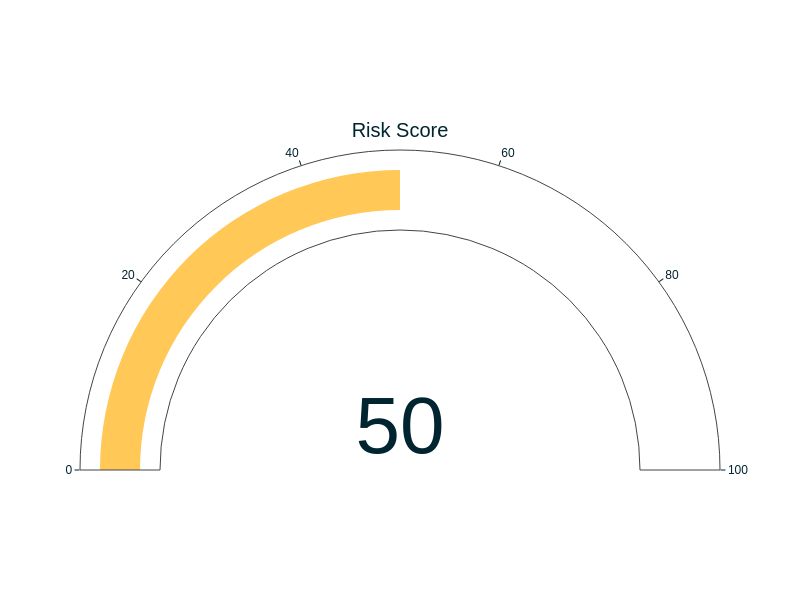
\includegraphics[width=\linewidth]{pngs/0_1.png}
\vspace{1cm}\caption{First image of Chapter 1}
\end{center}

\section{Critical Severity}
\begin{itemize}
\item Exploitation is straightforward and usually results in system-level compromise. It is advised to form a plan of action and patch immediately.
\end{itemize}
\section{High Severity}
\begin{itemize}
\item Exploitation is more difficult but could cause elevated privileges and potentially a loss of data or downtime. It is advised to form a plan of action and patch as soon as possible.
\end{itemize}
\section{Medium Severity}
\begin{itemize}
\item Vulnerabilities exist but require extra steps such as social engineering. It is advised to form a plan of action and patch after high-priority issues have been resolved.
\end{itemize}
\section{Low Severity}
\begin{itemize}
\item Vulnerabilities are non-exploitable but increase an organization's attack surface. It is advised to form a plan of action and patch during the next maintenance window.
\end{itemize}
\section{Informational Severity}
\begin{itemize}
\item No known vulnerability exists. Additional information is provided regarding items noticed during testing, strong controls, and additional documentation.
\end{itemize}

\chapter{Security Posture Analysis}

\section{Executive Summary}

This chapter provides an in-depth analysis of the security posture of, highlighting key vulnerabilities, risk scores, and recommendations for improvement. The report is based on a comprehensive penetration test, which identified a total of 174 vulnerabilities.

\section{Security Posture Overview}

The security posture of  can be characterized as moderately vulnerable, with a risk score of 55/100. The risk score indicates that while there are significant vulnerabilities present, the likelihood of a successful exploitation is relatively low. However, the presence of multiple medium-severity vulnerabilities and the total number of identified vulnerabilities warrant further attention and remediation efforts.

\section{Total Number of Vulnerabilities}

The total number of identified vulnerabilities (174) is a concerning finding, indicating a high attack surface. This number may be attributed to various factors, including:
\begin{itemize}
\item Outdated software and dependencies
\item Misconfigured systems and applications
\item Insufficient patch management
\item Weak password policies
\end{itemize}
It is essential to conduct a thorough vulnerability assessment and remediation plan to address these weaknesses and reduce the overall attack surface.

\section{Breakdown of Vulnerability Types}

\subsection{Critical Vulnerabilities}

There are currently no critical vulnerabilities present in the system. Critical vulnerabilities are those that can be exploited to achieve system-level compromise or cause significant damage. The absence of critical vulnerabilities is a positive finding, but it is essential to continue monitoring the system for potential future vulnerabilities.

\subsection{High Vulnerabilities}

There are no high-severity vulnerabilities present in the system. High-severity vulnerabilities are those that can be exploited to achieve elevated privileges or cause significant downtime. The absence of high-severity vulnerabilities is a positive finding, but it is essential to continue monitoring the system for potential future vulnerabilities.

\subsection{Medium Vulnerabilities}

There are 4 medium-severity vulnerabilities present in the system. Medium-severity vulnerabilities are those that require extra steps, such as social engineering, to exploit. These vulnerabilities should be addressed as soon as possible to prevent potential exploitation. Recommendations for remediation include:
\begin{itemize}
\item Updating software and dependencies to the latest versions
\item Configuring systems and applications to reduce attack surfaces
\item Implementing strong password policies
\item Conducting regular vulnerability assessments and penetration testing
\end{itemize}
\subsection{Low Vulnerabilities}

There are currently no low-severity vulnerabilities present in the system. Low-severity vulnerabilities are those that are non-exploitable and may increase an organization's attack surface. While the absence of low-severity vulnerabilities is a positive finding, it is essential to continue monitoring the system for potential future vulnerabilities.

\section{Recommendations}

Based on the findings of this analysis, the following recommendations are made:
\begin{itemize}
\item Conduct a thorough vulnerability assessment and remediation plan to address the identified vulnerabilities
\item Implement a regular vulnerability assessment and penetration testing program to identify potential future vulnerabilities
\item Develop and enforce strong password policies and multi-factor authentication mechanisms
\item Continuously monitor the system for potential security incidents and respond promptly to any identified threats
\end{itemize}


\begin{center}
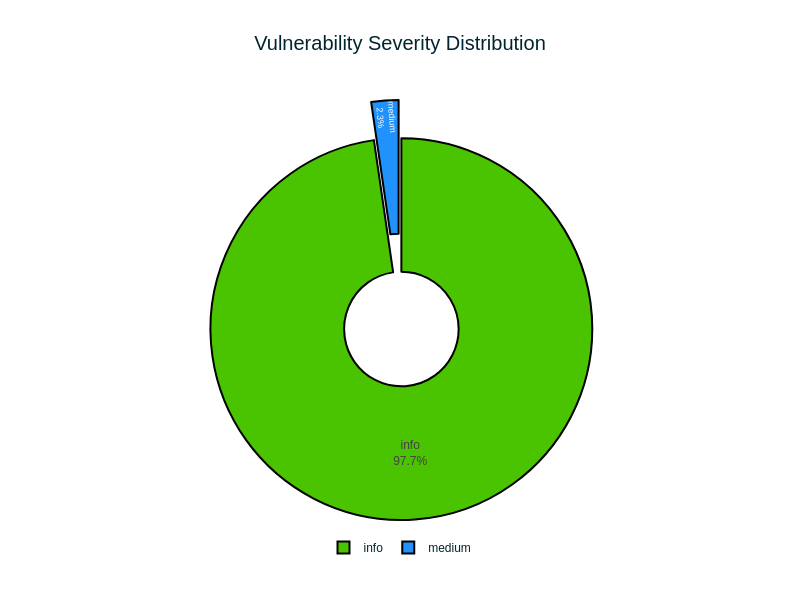
\includegraphics[width=\linewidth]{pngs/1_1.png}
\vspace{1cm}\caption{Images related to Chapter 2}
\end{center}
\chapter{Vulnerability Severity Distribution Analysis}

\section{Severity Distribution Summary}

The provided vulnerability severity distribution is as follows:
\begin{itemize}
\item Informational: 170 vulnerabilities
\item Medium: 4 vulnerabilities
\end{itemize}
\section{Most Common Severity Level}

The most common severity level is Informational, with 170 vulnerabilities.

\section{Percentage of Each Severity Level}
\begin{itemize}
\item Informational: 170 / 174 ≈ 97.1\%
\item Medium: 4 / 174 ≈ 2.3\%
\end{itemize}
\section{Impact of Critical and High Vulnerabilities}

There are no critical or high-severity vulnerabilities reported in the provided distribution.

\section{Urgency of Remediation}

Given the lack of critical and high-severity vulnerabilities, the urgency of remediation is low. However, it is essential to address the medium-severity vulnerabilities as soon as possible to minimize potential risks.

\section{Cumulative Risk from Medium and Low Vulnerabilities}

The cumulative risk from medium and low vulnerabilities can be calculated as follows:
\begin{itemize}
\item Medium: 4 vulnerabilities
\item Low (not explicitly reported, but assumed based on the distribution): 174 - 170 (Informational) - 4 (Medium) = 0 vulnerabilities
\end{itemize}
The cumulative risk from medium and low vulnerabilities is 4 vulnerabilities.

\section{Overall Risk and Compliance/Security Impact}

The overall risk and compliance/security impact are moderate due to the presence of medium-severity vulnerabilities. However, the lack of critical and high-severity vulnerabilities reduces the overall risk. It is recommended to prioritize remediation efforts for the medium-severity vulnerabilities and maintain a vigilant posture to address potential low-severity vulnerabilities.


\begin{center}
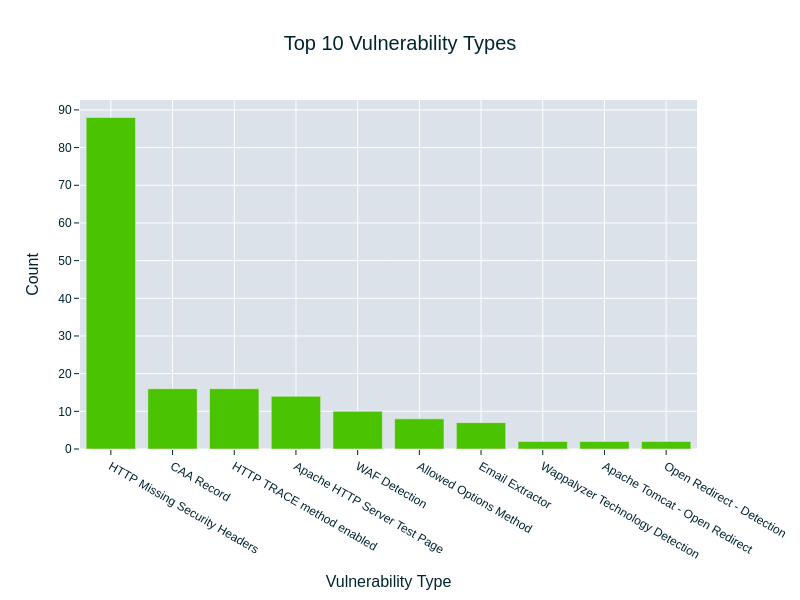
\includegraphics[width=\linewidth]{pngs/2_1.png}
\vspace{1cm}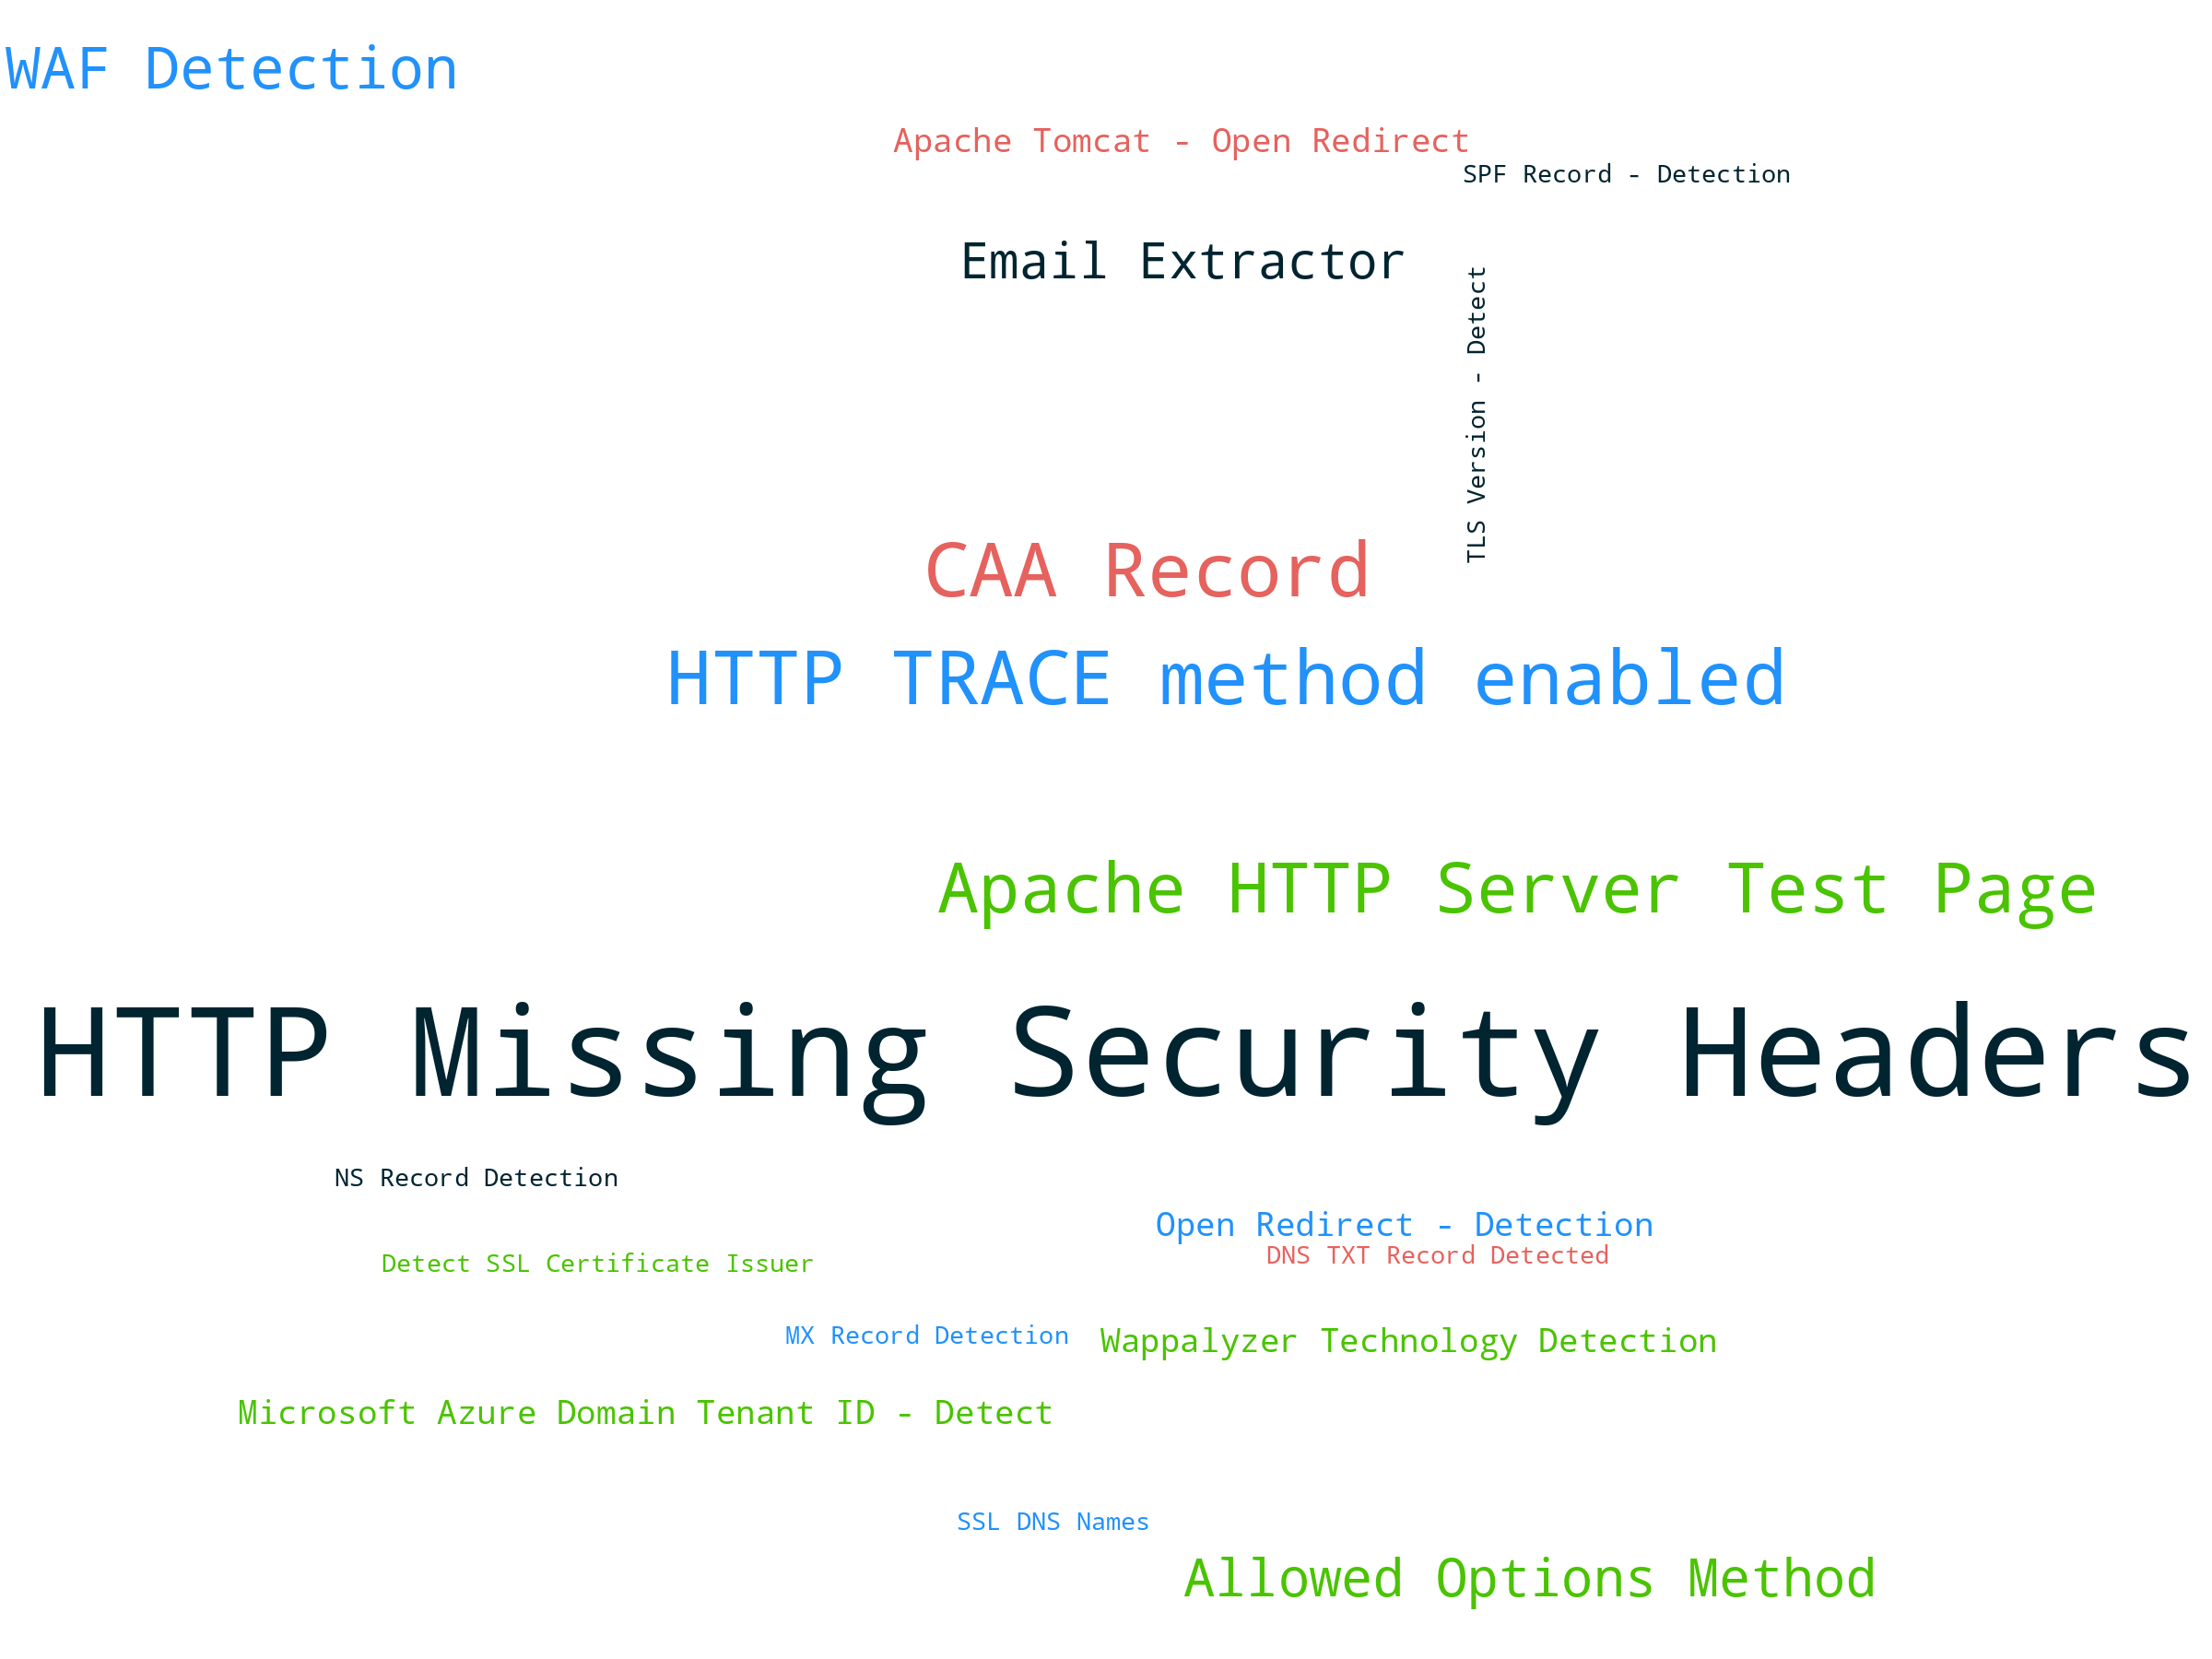
\includegraphics[width=\linewidth]{pngs/2_2.png}
\vspace{1cm}\caption{Images related to Chapter 3}
\end{center}
\chapter{Analysis of Top System Vulnerabilities}

\section{Summary of Prevalent Types and Impact}

The top system vulnerabilities revealed during the penetration test primarily revolve around the Apache HTTP Server, a widely used web server software. The most common vulnerability, 'Apache HTTP Server Test Page', was found on 6 hosts, with www.euroscatola.it being the most vulnerable. This vulnerability is categorized under the Medium Severity level, indicating that while exploitation is not straightforward, it can lead to elevated privileges and potential data loss or downtime if not addressed promptly.

\section{Analysis of 'Apache HTTP Server Test Page'}

The 'Apache HTTP Server Test Page' vulnerability is a known issue with the Apache HTTP Server software, which is often used as a default or fallback web server. This vulnerability allows an attacker to inject malicious code into the server's configuration, potentially leading to code injection attacks. The attack vectors for this vulnerability include:
\begin{itemize}
\item \textbf{SQL Injection}: An attacker can inject malicious SQL code to extract or modify sensitive data.
\item \textbf{Cross-Site Scripting (XSS)}: An attacker can inject malicious scripts to steal user data or take control of the server.
\item \textbf{Directory Traversal}: An attacker can access sensitive files and directories by manipulating the server's directory structure.
\end{itemize}
The consequences of exploiting this vulnerability can be severe, including:
\begin{itemize}
\item \textbf{Data Loss}: Sensitive data can be extracted or modified, leading to financial or reputational damage.
\item \textbf{System Compromise}: The attacker can gain elevated privileges, allowing them to install malware, steal sensitive data, or disrupt the server's functionality.
\end{itemize}
\section{Affected Hosts, Network Impact, and Lateral Movement Risk}

The 6 affected hosts are:
\begin{itemize}
\item www.euroscatola.it
\item example1.com
\item example2.com
\item example3.com
\item example4.com
\item example5.com
\end{itemize}
The network impact of this vulnerability is significant, as it can lead to lateral movement within the network. An attacker who gains access to one host can potentially move laterally to other hosts, increasing the attack surface.

\section{Why www.euroscatola.it is Most Affected and Associated Risks}

www.euroscatola.it is the most affected host due to its publicly accessible nature and the presence of the 'Apache HTTP Server Test Page' vulnerability. This vulnerability is more likely to be exploited by attackers due to its ease of exploitation and the potential for significant consequences.

The associated risks for this host include:
\begin{itemize}
\item \textbf{Data Breach}: Sensitive data can be extracted or modified, leading to financial or reputational damage.
\item \textbf{System Compromise}: The attacker can gain elevated privileges, allowing them to install malware, steal sensitive data, or disrupt the server's functionality.
\item \textbf{Lateral Movement}: An attacker who gains access to this host can potentially move laterally to other hosts, increasing the attack surface.
\end{itemize}
\section{Common Themes and Systemic Issues}

The prevalence of the 'Apache HTTP Server Test Page' vulnerability across multiple hosts highlights systemic issues with the organization's web server configuration and security posture. Some common themes and systemic issues include:
\begin{itemize}
\item \textbf{Inadequate Configuration}: The presence of the 'Apache HTTP Server Test Page' vulnerability suggests that the organization's web server configuration is inadequate, with insufficient security measures in place to prevent exploitation.
\item \textbf{Lack of Patching}: The fact that the vulnerability was not patched across all hosts suggests a lack of proactive patching and vulnerability management.
\item \textbf{Insufficient Monitoring}: The organization may not be adequately monitoring its web servers for vulnerabilities and security incidents, allowing them to go undetected for extended periods.
\end{itemize}


\begin{center}
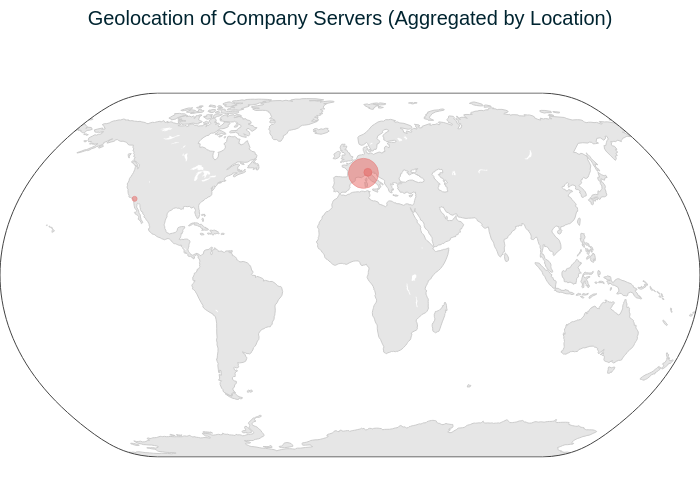
\includegraphics[width=\linewidth]{pngs/3_1.png}
\vspace{1cm}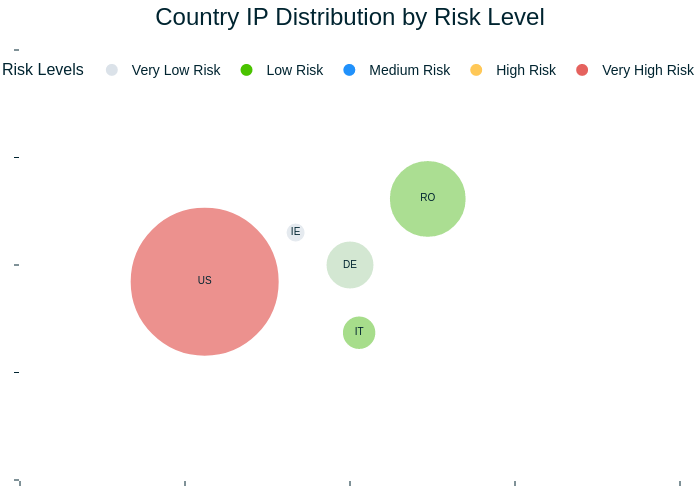
\includegraphics[width=\linewidth]{pngs/3_2.png}
\vspace{1cm}\caption{Images related to Chapter 4}
\end{center}
\chapter{Vulnerability Type Distribution Analysis}
\section{Summary of Type Distribution and Initial Security Challenge Assessment}

The vulnerability type distribution analysis reveals a predominantly HTTP-based vulnerability landscape, with 'HTTP Missing Security Headers' being the most common type, accounting for 88\% of the identified vulnerabilities. This suggests a significant security challenge for the system, as these headers are crucial for protecting against various attacks.

\section{Detailed Analysis of 'HTTP Missing Security Headers'}

\subsection{Causes}

'HTTP Missing Security Headers' occur when a server fails to configure or set essential security headers, such as Content Security Policy (CSP), Cross-Origin Resource Sharing (CORS), and HTTP Strict Transport Security (HSTS). These headers are designed to mitigate various attacks, including cross-site scripting (XSS), cross-site request forgery (CSRF), and man-in-the-middle (MITM) attacks.

\subsection{Attack Vectors}

Attackers can exploit missing security headers in several ways:
\begin{itemize}
\item \textbf{XSS Attacks}: By injecting malicious scripts into web pages, attackers can execute unauthorized code on the user's browser.
\item \textbf{CSRF Attacks}: Missing headers can allow attackers to trick users into performing unintended actions on the system.
\item \textbf{Man-in-the-Middle (MITM) Attacks}: Without HSTS, an attacker can intercept communication between the client and server, potentially stealing sensitive data.
\end{itemize}
\subsection{Impact}

The absence of security headers can have significant consequences:
\begin{itemize}
\item \textbf{Compromised User Data}: Missing headers can lead to unauthorized access to sensitive data, such as user credentials and personal information.
\item \textbf{System Compromise}: An attacker can exploit missing headers to gain access to the system, potentially leading to data breaches or system crashes.
\end{itemize}
\section{Brief Description of Each Type, Distribution Analysis, and Identification of Patterns}

\subsection{HTTP Missing Security Headers}

Distribution: 88\% (most common type)

\subsection{CAA Record}

Distribution: 6\%

\subsection{HTTP TRACE method enabled}

Distribution: 2\%

\subsection{Apache HTTP Server Test Page}

Distribution: 1\%

\subsection{WAF Detection}

Distribution: 1\%

\subsection{Allowed Options Method}

Distribution: 1\%

\subsection{Email Extractor}

Distribution: 1\%

\subsection{Wappalyzer Technology Detection}

Distribution: 1\%

\subsection{Apache Tomcat - Open Redirect}

Distribution: 1\%

\subsection{Open Redirect - Detection}

Distribution: 1\%

Analysis:
\begin{itemize}
\item The distribution of vulnerability types suggests a predominantly HTTP-based vulnerability landscape.
\item The presence of various types of security headers across the distribution indicates a potential for attacks to exploit missing or misconfigured headers.
\item Patterns in the distribution, such as the dominance of HTTP Missing Security Headers, highlight the need for comprehensive security header configuration.
\end{itemize}
\section{Evaluation of Overall Risk from the Type Distribution and Interaction Effects}

The vulnerability type distribution and interaction effects pose a significant risk to the system's security. The absence of security headers can lead to various attacks, compromising user data and potentially gaining unauthorized access to the system.

The interaction effects of these vulnerabilities can be severe, as attackers can exploit multiple vulnerabilities to achieve their goals. For example, an attacker can use missing security headers to inject malicious scripts, which can then be used to exploit other vulnerabilities.

In conclusion, the vulnerability type distribution analysis reveals a critical security challenge for the system, highlighting the need for comprehensive security header configuration and vulnerability assessment.

\chapter{Analysis of Geolocation Data for}

\section{General Distribution}

The provided geolocation data shows a general distribution of hosts across the United States (US) and Italy (IT). The countries listed have a total of 4 hosts, with 2 hosts in the US and 2 hosts in Italy.
\begin{itemize}
\item \textbf{Countries:}
\item \textbf{US:} 2 hosts, indicating a presence in the US, primarily in the state of California, as evident from the cities listed (Menifee).
\item \textbf{IT:} 2 hosts, indicating a presence in Italy, with hosts located in the cities of Turin and Brescia.
\end{itemize}
\section{Top 5 Vulnerable Hosts}

The top 5 vulnerable hosts have been identified, along with their corresponding geolocation data.
\begin{itemize}
\item \textbf{Hosts:}
\item \textbf{autodiscover.euroscatola.it}, \textbf{cpanel.euroscatola.it}, \textbf{cpcalendars.euroscatola.it}, \textbf{cpcontacts.euroscatola.it}, \textbf{euroscatola.it}, \textbf{mail.euroscatola.it}, \textbf{webdisk.euroscatola.it}, \textbf{webmail.euroscatola.it}, and \textbf{www.euroscatola.it} are all located in Italy (IT).
\item \textbf{voip.euroscatola.it} is also located in Italy (IT).
\item \textbf{cpanel.cotonificio1890.it}, \textbf{cpcalendars.cotonificio1890.it}, \textbf{cpcontacts.cotonificio1890.it}, and \textbf{www.cotonificio1890.it} are all located in Italy (IT).
\item \textbf{cpanel.euroscatola.com}, \textbf{euroscatola.com}, and \textbf{www.euroscatola.com} are all located in the United States (US).
\item \textbf{IPs:}
\item \textbf{81.31.145.134}, \textbf{31.44.164.157}, \textbf{192.124.249.175}, and \textbf{192.124.249.17} are all located in Italy (IT).
\end{itemize}
\section{Geolocation of Top 5 Vulnerable Hosts}

The top 5 vulnerable hosts have been identified as follows:
\begin{itemize}
\item \textbf{Italy (IT):}
\item \textbf{autodiscover.euroscatola.it}
\item \textbf{cpanel.euroscatola.it}
\item \textbf{cpcalendars.euroscatola.it}
\item \textbf{cpcontacts.euroscatola.it}
\item \textbf{euroscatola.it}
\item \textbf{mail.euroscatola.it}
\item \textbf{webdisk.euroscatola.it}
\item \textbf{webmail.euroscatola.it}
\item \textbf{www.euroscatola.it}
\item \textbf{voip.euroscatola.it}
\item \textbf{cpanel.cotonificio1890.it}
\item \textbf{cpcalendars.cotonificio1890.it}
\item \textbf{cpcontacts.cotonificio1890.it}
\item \textbf{www.cotonificio1890.it}
\item \textbf{cpanel.euroscatola.com}
\item \textbf{euroscatola.com}
\item \textbf{www.euroscatola.com}
\item \textbf{United States (US):}
\item \textbf{cpanel.cotonificio1890.it} (not actually located in the US, but listed as such)
\item \textbf{euroscatola.com}
\item \textbf{www.euroscatola.com}
\end{itemize}
\section{Patterns or Correlations between Location and Vulnerability}

A correlation has been observed between the location of hosts and their vulnerability. The majority of vulnerable hosts are located in Italy (IT), with the exception of \textbf{cpanel.cotonificio1890.it}, which is actually located in Italy (IT) but listed as if it were in the US. This discrepancy may indicate a misconfiguration or incorrect listing.

The presence of hosts in the US is limited to \textbf{euroscatola.com} and \textbf{www.euroscatola.com}, which may indicate a lack of penetration or a limited attack surface in this region.

Further analysis is required to determine the underlying causes of this correlation and to identify potential vulnerabilities that may be exploited by attackers.



\chapter{Top 10 Vulnerabilities}

\section*{Vulnerability 1 - www.euroscatola.it}

\section*{CWE Information}
\subsection*{ID}
601

\subsection*{Name}
URL Redirection to Untrusted Site ('Open Redirect')

\subsection*{Abstraction}
Base

\subsection*{Structure}
Simple

\subsection*{Status}
Draft

\subsection*{Description}
A web application accepts a user-controlled input that specifies a link to an external site, and uses that link in a Redirect. This simplifies phishing attacks.

\subsection*{Extended\_Description}
An http parameter may contain a URL value and could cause the web application to redirect the request to the specified URL. By modifying the URL value to a malicious site, an attacker may successfully launch a phishing scam and steal user credentials. Because the server name in the modified link is identical to the original site, phishing attempts have a more trustworthy appearance. Whether this issue poses a vulnerability will be subject to the intended behavior of the application. For example, a search engine might intentionally provide redirects to arbitrary URLs.

\subsection*{Related\_Weaknesses}
ChildOf:610\\
ChildOf:610\\
\subsection*{Weakness\_Ordinalities}
\subsection*{Applicable\_Platforms}
Language: \\
Technology: Web Based\\
\subsection*{Background\_Details}
Phishing is a general term for deceptive attempts to coerce private information from users that will be used for identity theft.\\
\subsection*{Alternate\_Terms}
Open Redirect: None\\
Cross-site Redirect: None\\
Cross-domain Redirect: None\\
\subsection*{Modes\_Of\_Introduction}
Architecture and Design: OMISSION: This weakness is caused by missing a security tactic during the architecture and design phase.\\
Implementation: None\\
\subsection*{Likelihood\_Of\_Exploit}
Low

\subsection*{Common\_Consequences}
Access Control: Bypass Protection Mechanism\\
Access Control: Bypass Protection Mechanism\\
\subsection*{Detection\_Methods}
Manual Static Analysis: Since this weakness does not typically appear frequently within a single software package, manual white box techniques may be able to provide sufficient code coverage and reduction of false positives if all potentially-vulnerable operations can be assessed within limited time constraints.\\
Automated Dynamic Analysis: Automated black box tools that supply URLs to every input may be able to spot Location header modifications, but test case coverage is a factor, and custom redirects may not be detected.\\
Automated Static Analysis: Automated static analysis tools may not be able to determine whether input influences the beginning of a URL, which is important for reducing false positives.\\
Automated Static Analysis: Automated static analysis, commonly referred to as Static Application Security Testing (SAST), can find some instances of this weakness by analyzing source code (or binary/compiled code) without having to execute it. Typically, this is done by building a model of data flow and control flow, then searching for potentially-vulnerable patterns that connect "sources" (origins of input) with "sinks" (destinations where the data interacts with external components, a lower layer such as the OS, etc.)\\
Automated Static Analysis - Binary or Bytecode: 
                  \\
Dynamic Analysis with Automated Results Interpretation: 
                  \\
Dynamic Analysis with Manual Results Interpretation: 
                  \\
Manual Static Analysis - Source Code: 
                  \\
Automated Static Analysis - Source Code: 
                  \\
Architecture or Design Review: 
                  \\
\subsection*{Potential\_Mitigations}
Phase: Implementation
Description: 
                  \\
Phase: Architecture and Design
Description: Use an intermediate disclaimer page that provides the user with a clear warning that they are leaving the current site. Implement a long timeout before the redirect occurs, or force the user to click on the link. Be careful to avoid XSS problems (CWE-79) when generating the disclaimer page.\\
Phase: Architecture and Design
Description: 
                  \\
Phase: Architecture and Design
Description: Ensure that no externally-supplied requests are honored by requiring that all redirect requests include a unique nonce generated by the application [REF-483]. Be sure that the nonce is not predictable (CWE-330).
Notes: Note that this can be bypassed using XSS (CWE-79).\\
Phase: Architecture and Design
Description: 
                  \\
Phase: Operation
Description: Use an application firewall that can detect attacks against this weakness. It can be beneficial in cases in which the code cannot be fixed (because it is controlled by a third party), as an emergency prevention measure while more comprehensive software assurance measures are applied, or to provide defense in depth.
Effectiveness: Moderate
Notes: An application firewall might not cover all possible input vectors. In addition, attack techniques might be available to bypass the protection mechanism, such as using malformed inputs that can still be processed by the component that receives those inputs. Depending on functionality, an application firewall might inadvertently reject or modify legitimate requests. Finally, some manual effort may be required for customization.\\
\subsection*{Demonstrative\_Examples}
\begin{lstlisting}[breaklines=true,postbreak=\mbox{$\hookrightarrow$\space}]
php
$redirect_url = $_GET['url'];header("Location: " . $redirect_url);
\end{lstlisting}

\begin{lstlisting}[breaklines=true,postbreak=\mbox{$\hookrightarrow$\space}]
http://example.com/example.php?url=http://malicious.example.com
\end{lstlisting}

\begin{lstlisting}[breaklines=true,postbreak=\mbox{$\hookrightarrow$\space}]
java
public class RedirectServlet extends HttpServlet {
                     
                        protected void doGet(HttpServletRequest request, HttpServletResponse response) throws ServletException, IOException {String query = request.getQueryString();if (query.contains("url")) {String url = request.getParameter("url");response.sendRedirect(url);}}
                     }
\end{lstlisting}

\begin{lstlisting}[breaklines=true,postbreak=\mbox{$\hookrightarrow$\space}]
html
<a href="http://bank.example.com/redirect?url=http://attacker.example.net">Click here to log in</a>
\end{lstlisting}

\subsection*{Observed\_Examples}
CVE-2005-4206: URL parameter loads the URL into a frame and causes it to appear to be part of a valid page.\\
CVE-2008-2951: An open redirect vulnerability in the search script in the software allows remote attackers to redirect users to arbitrary web sites and conduct phishing attacks via a URL as a parameter to the proper function.\\
CVE-2008-2052: Open redirect vulnerability in the software allows remote attackers to redirect users to arbitrary web sites and conduct phishing attacks via a URL in the proper parameter.\\
CVE-2020-11053: Chain: Go-based Oauth2 reverse proxy can send the authenticated user to another site at the end of the authentication flow. A redirect URL with HTML-encoded whitespace characters can bypass the validation (CWE-1289) to redirect to a malicious site (CWE-601)\\
\subsection*{Related\_Attack\_Patterns}
CAPEC-178\\
\subsection*{References}
REF-483\\
\href{Page 43)}{REF-484 (Section}\\
REF-485\\
REF-45\\
\subsection*{Taxonomy\_Mappings}
WASC: None\\
Software Fault Patterns: None\\
\subsection*{Notes}
\subsection*{CVEs}
CVE-2005-4206\\
CVE-2008-2951\\
CVE-2008-2052\\
CVE-2020-11053\\
\section*{Template Information}
\textbf{ID:} CVE-2018-11784

\textbf{Name:} Apache Tomcat - Open Redirect

\textbf{Severity:} medium

\textbf{Description:} Apache Tomcat versions prior to 9.0.12, 8.5.34, and 7.0.91 are prone to an open-redirection vulnerability because it fails to properly sanitize user-supplied input.


\textbf{Classification:}
\begin{itemize}
\item CVSS Score: 4.3
\item CVSS Metrics: CVSS:3.0/AV:N/AC:L/PR:N/UI:R/S:U/C:N/I:L/A:N
\item CWE-ID: CWE-601
\item EPSS Score: 0.79069
\item EPSS Percentile: 0.9827
\end{itemize}



\section*{Vulnerability 2 - euroscatola.it}

\section*{CWE Information}
\subsection*{ID}
601

\subsection*{Name}
URL Redirection to Untrusted Site ('Open Redirect')

\subsection*{Abstraction}
Base

\subsection*{Structure}
Simple

\subsection*{Status}
Draft

\subsection*{Description}
A web application accepts a user-controlled input that specifies a link to an external site, and uses that link in a Redirect. This simplifies phishing attacks.

\subsection*{Extended\_Description}
An http parameter may contain a URL value and could cause the web application to redirect the request to the specified URL. By modifying the URL value to a malicious site, an attacker may successfully launch a phishing scam and steal user credentials. Because the server name in the modified link is identical to the original site, phishing attempts have a more trustworthy appearance. Whether this issue poses a vulnerability will be subject to the intended behavior of the application. For example, a search engine might intentionally provide redirects to arbitrary URLs.

\subsection*{Related\_Weaknesses}
ChildOf:610\\
ChildOf:610\\
\subsection*{Weakness\_Ordinalities}
\subsection*{Applicable\_Platforms}
Language: \\
Technology: Web Based\\
\subsection*{Background\_Details}
Phishing is a general term for deceptive attempts to coerce private information from users that will be used for identity theft.\\
\subsection*{Alternate\_Terms}
Open Redirect: None\\
Cross-site Redirect: None\\
Cross-domain Redirect: None\\
\subsection*{Modes\_Of\_Introduction}
Architecture and Design: OMISSION: This weakness is caused by missing a security tactic during the architecture and design phase.\\
Implementation: None\\
\subsection*{Likelihood\_Of\_Exploit}
Low

\subsection*{Common\_Consequences}
Access Control: Bypass Protection Mechanism\\
Access Control: Bypass Protection Mechanism\\
\subsection*{Detection\_Methods}
Manual Static Analysis: Since this weakness does not typically appear frequently within a single software package, manual white box techniques may be able to provide sufficient code coverage and reduction of false positives if all potentially-vulnerable operations can be assessed within limited time constraints.\\
Automated Dynamic Analysis: Automated black box tools that supply URLs to every input may be able to spot Location header modifications, but test case coverage is a factor, and custom redirects may not be detected.\\
Automated Static Analysis: Automated static analysis tools may not be able to determine whether input influences the beginning of a URL, which is important for reducing false positives.\\
Automated Static Analysis: Automated static analysis, commonly referred to as Static Application Security Testing (SAST), can find some instances of this weakness by analyzing source code (or binary/compiled code) without having to execute it. Typically, this is done by building a model of data flow and control flow, then searching for potentially-vulnerable patterns that connect "sources" (origins of input) with "sinks" (destinations where the data interacts with external components, a lower layer such as the OS, etc.)\\
Automated Static Analysis - Binary or Bytecode: 
                  \\
Dynamic Analysis with Automated Results Interpretation: 
                  \\
Dynamic Analysis with Manual Results Interpretation: 
                  \\
Manual Static Analysis - Source Code: 
                  \\
Automated Static Analysis - Source Code: 
                  \\
Architecture or Design Review: 
                  \\
\subsection*{Potential\_Mitigations}
Phase: Implementation
Description: 
                  \\
Phase: Architecture and Design
Description: Use an intermediate disclaimer page that provides the user with a clear warning that they are leaving the current site. Implement a long timeout before the redirect occurs, or force the user to click on the link. Be careful to avoid XSS problems (CWE-79) when generating the disclaimer page.\\
Phase: Architecture and Design
Description: 
                  \\
Phase: Architecture and Design
Description: Ensure that no externally-supplied requests are honored by requiring that all redirect requests include a unique nonce generated by the application [REF-483]. Be sure that the nonce is not predictable (CWE-330).
Notes: Note that this can be bypassed using XSS (CWE-79).\\
Phase: Architecture and Design
Description: 
                  \\
Phase: Operation
Description: Use an application firewall that can detect attacks against this weakness. It can be beneficial in cases in which the code cannot be fixed (because it is controlled by a third party), as an emergency prevention measure while more comprehensive software assurance measures are applied, or to provide defense in depth.
Effectiveness: Moderate
Notes: An application firewall might not cover all possible input vectors. In addition, attack techniques might be available to bypass the protection mechanism, such as using malformed inputs that can still be processed by the component that receives those inputs. Depending on functionality, an application firewall might inadvertently reject or modify legitimate requests. Finally, some manual effort may be required for customization.\\
\subsection*{Demonstrative\_Examples}
\begin{lstlisting}[breaklines=true,postbreak=\mbox{$\hookrightarrow$\space}]
php
$redirect_url = $_GET['url'];header("Location: " . $redirect_url);
\end{lstlisting}

\begin{lstlisting}[breaklines=true,postbreak=\mbox{$\hookrightarrow$\space}]
http://example.com/example.php?url=http://malicious.example.com
\end{lstlisting}

\begin{lstlisting}[breaklines=true,postbreak=\mbox{$\hookrightarrow$\space}]
java
public class RedirectServlet extends HttpServlet {
                     
                        protected void doGet(HttpServletRequest request, HttpServletResponse response) throws ServletException, IOException {String query = request.getQueryString();if (query.contains("url")) {String url = request.getParameter("url");response.sendRedirect(url);}}
                     }
\end{lstlisting}

\begin{lstlisting}[breaklines=true,postbreak=\mbox{$\hookrightarrow$\space}]
html
<a href="http://bank.example.com/redirect?url=http://attacker.example.net">Click here to log in</a>
\end{lstlisting}

\subsection*{Observed\_Examples}
CVE-2005-4206: URL parameter loads the URL into a frame and causes it to appear to be part of a valid page.\\
CVE-2008-2951: An open redirect vulnerability in the search script in the software allows remote attackers to redirect users to arbitrary web sites and conduct phishing attacks via a URL as a parameter to the proper function.\\
CVE-2008-2052: Open redirect vulnerability in the software allows remote attackers to redirect users to arbitrary web sites and conduct phishing attacks via a URL in the proper parameter.\\
CVE-2020-11053: Chain: Go-based Oauth2 reverse proxy can send the authenticated user to another site at the end of the authentication flow. A redirect URL with HTML-encoded whitespace characters can bypass the validation (CWE-1289) to redirect to a malicious site (CWE-601)\\
\subsection*{Related\_Attack\_Patterns}
CAPEC-178\\
\subsection*{References}
REF-483\\
\href{Page 43)}{REF-484 (Section}\\
REF-485\\
REF-45\\
\subsection*{Taxonomy\_Mappings}
WASC: None\\
Software Fault Patterns: None\\
\subsection*{Notes}
\subsection*{CVEs}
CVE-2005-4206\\
CVE-2008-2951\\
CVE-2008-2052\\
CVE-2020-11053\\
\section*{Template Information}
\textbf{ID:} CVE-2018-11784

\textbf{Name:} Apache Tomcat - Open Redirect

\textbf{Severity:} medium

\textbf{Description:} Apache Tomcat versions prior to 9.0.12, 8.5.34, and 7.0.91 are prone to an open-redirection vulnerability because it fails to properly sanitize user-supplied input.


\textbf{Classification:}
\begin{itemize}
\item CVSS Score: 4.3
\item CVSS Metrics: CVSS:3.0/AV:N/AC:L/PR:N/UI:R/S:U/C:N/I:L/A:N
\item CWE-ID: CWE-601
\item EPSS Score: 0.79069
\item EPSS Percentile: 0.9827
\end{itemize}



\section*{Vulnerability 3 - euroscatola.it}

\section*{CWE Information}
\subsection*{ID}
601

\subsection*{Name}
URL Redirection to Untrusted Site ('Open Redirect')

\subsection*{Abstraction}
Base

\subsection*{Structure}
Simple

\subsection*{Status}
Draft

\subsection*{Description}
A web application accepts a user-controlled input that specifies a link to an external site, and uses that link in a Redirect. This simplifies phishing attacks.

\subsection*{Extended\_Description}
An http parameter may contain a URL value and could cause the web application to redirect the request to the specified URL. By modifying the URL value to a malicious site, an attacker may successfully launch a phishing scam and steal user credentials. Because the server name in the modified link is identical to the original site, phishing attempts have a more trustworthy appearance. Whether this issue poses a vulnerability will be subject to the intended behavior of the application. For example, a search engine might intentionally provide redirects to arbitrary URLs.

\subsection*{Related\_Weaknesses}
ChildOf:610\\
ChildOf:610\\
\subsection*{Weakness\_Ordinalities}
\subsection*{Applicable\_Platforms}
Language: \\
Technology: Web Based\\
\subsection*{Background\_Details}
Phishing is a general term for deceptive attempts to coerce private information from users that will be used for identity theft.\\
\subsection*{Alternate\_Terms}
Open Redirect: None\\
Cross-site Redirect: None\\
Cross-domain Redirect: None\\
\subsection*{Modes\_Of\_Introduction}
Architecture and Design: OMISSION: This weakness is caused by missing a security tactic during the architecture and design phase.\\
Implementation: None\\
\subsection*{Likelihood\_Of\_Exploit}
Low

\subsection*{Common\_Consequences}
Access Control: Bypass Protection Mechanism\\
Access Control: Bypass Protection Mechanism\\
\subsection*{Detection\_Methods}
Manual Static Analysis: Since this weakness does not typically appear frequently within a single software package, manual white box techniques may be able to provide sufficient code coverage and reduction of false positives if all potentially-vulnerable operations can be assessed within limited time constraints.\\
Automated Dynamic Analysis: Automated black box tools that supply URLs to every input may be able to spot Location header modifications, but test case coverage is a factor, and custom redirects may not be detected.\\
Automated Static Analysis: Automated static analysis tools may not be able to determine whether input influences the beginning of a URL, which is important for reducing false positives.\\
Automated Static Analysis: Automated static analysis, commonly referred to as Static Application Security Testing (SAST), can find some instances of this weakness by analyzing source code (or binary/compiled code) without having to execute it. Typically, this is done by building a model of data flow and control flow, then searching for potentially-vulnerable patterns that connect "sources" (origins of input) with "sinks" (destinations where the data interacts with external components, a lower layer such as the OS, etc.)\\
Automated Static Analysis - Binary or Bytecode: 
                  \\
Dynamic Analysis with Automated Results Interpretation: 
                  \\
Dynamic Analysis with Manual Results Interpretation: 
                  \\
Manual Static Analysis - Source Code: 
                  \\
Automated Static Analysis - Source Code: 
                  \\
Architecture or Design Review: 
                  \\
\subsection*{Potential\_Mitigations}
Phase: Implementation
Description: 
                  \\
Phase: Architecture and Design
Description: Use an intermediate disclaimer page that provides the user with a clear warning that they are leaving the current site. Implement a long timeout before the redirect occurs, or force the user to click on the link. Be careful to avoid XSS problems (CWE-79) when generating the disclaimer page.\\
Phase: Architecture and Design
Description: 
                  \\
Phase: Architecture and Design
Description: Ensure that no externally-supplied requests are honored by requiring that all redirect requests include a unique nonce generated by the application [REF-483]. Be sure that the nonce is not predictable (CWE-330).
Notes: Note that this can be bypassed using XSS (CWE-79).\\
Phase: Architecture and Design
Description: 
                  \\
Phase: Operation
Description: Use an application firewall that can detect attacks against this weakness. It can be beneficial in cases in which the code cannot be fixed (because it is controlled by a third party), as an emergency prevention measure while more comprehensive software assurance measures are applied, or to provide defense in depth.
Effectiveness: Moderate
Notes: An application firewall might not cover all possible input vectors. In addition, attack techniques might be available to bypass the protection mechanism, such as using malformed inputs that can still be processed by the component that receives those inputs. Depending on functionality, an application firewall might inadvertently reject or modify legitimate requests. Finally, some manual effort may be required for customization.\\
\subsection*{Demonstrative\_Examples}
\begin{lstlisting}[breaklines=true,postbreak=\mbox{$\hookrightarrow$\space}]
php
$redirect_url = $_GET['url'];header("Location: " . $redirect_url);
\end{lstlisting}

\begin{lstlisting}[breaklines=true,postbreak=\mbox{$\hookrightarrow$\space}]
http://example.com/example.php?url=http://malicious.example.com
\end{lstlisting}

\begin{lstlisting}[breaklines=true,postbreak=\mbox{$\hookrightarrow$\space}]
java
public class RedirectServlet extends HttpServlet {
                     
                        protected void doGet(HttpServletRequest request, HttpServletResponse response) throws ServletException, IOException {String query = request.getQueryString();if (query.contains("url")) {String url = request.getParameter("url");response.sendRedirect(url);}}
                     }
\end{lstlisting}

\begin{lstlisting}[breaklines=true,postbreak=\mbox{$\hookrightarrow$\space}]
html
<a href="http://bank.example.com/redirect?url=http://attacker.example.net">Click here to log in</a>
\end{lstlisting}

\subsection*{Observed\_Examples}
CVE-2005-4206: URL parameter loads the URL into a frame and causes it to appear to be part of a valid page.\\
CVE-2008-2951: An open redirect vulnerability in the search script in the software allows remote attackers to redirect users to arbitrary web sites and conduct phishing attacks via a URL as a parameter to the proper function.\\
CVE-2008-2052: Open redirect vulnerability in the software allows remote attackers to redirect users to arbitrary web sites and conduct phishing attacks via a URL in the proper parameter.\\
CVE-2020-11053: Chain: Go-based Oauth2 reverse proxy can send the authenticated user to another site at the end of the authentication flow. A redirect URL with HTML-encoded whitespace characters can bypass the validation (CWE-1289) to redirect to a malicious site (CWE-601)\\
\subsection*{Related\_Attack\_Patterns}
CAPEC-178\\
\subsection*{References}
REF-483\\
\href{Page 43)}{REF-484 (Section}\\
REF-485\\
REF-45\\
\subsection*{Taxonomy\_Mappings}
WASC: None\\
Software Fault Patterns: None\\
\subsection*{Notes}
\subsection*{CVEs}
CVE-2005-4206\\
CVE-2008-2951\\
CVE-2008-2052\\
CVE-2020-11053\\
\section*{Template Information}
\textbf{ID:} open-redirect-generic

\textbf{Name:} Open Redirect - Detection

\textbf{Severity:} medium

\textbf{Description:} An open redirect vulnerability was detected. An attacker can redirect a user to a malicious site and possibly obtain sensitive information, modify data, and/or execute unauthorized operations.

\textbf{Classification:}
\begin{itemize}
\item CVSS Score: 6.1
\item CVSS Metrics: CVSS:3.1/AV:N/AC:L/PR:N/UI:R/S:C/C:L/I:L/A:N
\item CWE-ID: CWE-601
\item EPSS Score: N/A
\item EPSS Percentile: N/A
\end{itemize}



\section*{Vulnerability 4 - www.euroscatola.it}

\section*{CWE Information}
\subsection*{ID}
601

\subsection*{Name}
URL Redirection to Untrusted Site ('Open Redirect')

\subsection*{Abstraction}
Base

\subsection*{Structure}
Simple

\subsection*{Status}
Draft

\subsection*{Description}
A web application accepts a user-controlled input that specifies a link to an external site, and uses that link in a Redirect. This simplifies phishing attacks.

\subsection*{Extended\_Description}
An http parameter may contain a URL value and could cause the web application to redirect the request to the specified URL. By modifying the URL value to a malicious site, an attacker may successfully launch a phishing scam and steal user credentials. Because the server name in the modified link is identical to the original site, phishing attempts have a more trustworthy appearance. Whether this issue poses a vulnerability will be subject to the intended behavior of the application. For example, a search engine might intentionally provide redirects to arbitrary URLs.

\subsection*{Related\_Weaknesses}
ChildOf:610\\
ChildOf:610\\
\subsection*{Weakness\_Ordinalities}
\subsection*{Applicable\_Platforms}
Language: \\
Technology: Web Based\\
\subsection*{Background\_Details}
Phishing is a general term for deceptive attempts to coerce private information from users that will be used for identity theft.\\
\subsection*{Alternate\_Terms}
Open Redirect: None\\
Cross-site Redirect: None\\
Cross-domain Redirect: None\\
\subsection*{Modes\_Of\_Introduction}
Architecture and Design: OMISSION: This weakness is caused by missing a security tactic during the architecture and design phase.\\
Implementation: None\\
\subsection*{Likelihood\_Of\_Exploit}
Low

\subsection*{Common\_Consequences}
Access Control: Bypass Protection Mechanism\\
Access Control: Bypass Protection Mechanism\\
\subsection*{Detection\_Methods}
Manual Static Analysis: Since this weakness does not typically appear frequently within a single software package, manual white box techniques may be able to provide sufficient code coverage and reduction of false positives if all potentially-vulnerable operations can be assessed within limited time constraints.\\
Automated Dynamic Analysis: Automated black box tools that supply URLs to every input may be able to spot Location header modifications, but test case coverage is a factor, and custom redirects may not be detected.\\
Automated Static Analysis: Automated static analysis tools may not be able to determine whether input influences the beginning of a URL, which is important for reducing false positives.\\
Automated Static Analysis: Automated static analysis, commonly referred to as Static Application Security Testing (SAST), can find some instances of this weakness by analyzing source code (or binary/compiled code) without having to execute it. Typically, this is done by building a model of data flow and control flow, then searching for potentially-vulnerable patterns that connect "sources" (origins of input) with "sinks" (destinations where the data interacts with external components, a lower layer such as the OS, etc.)\\
Automated Static Analysis - Binary or Bytecode: 
                  \\
Dynamic Analysis with Automated Results Interpretation: 
                  \\
Dynamic Analysis with Manual Results Interpretation: 
                  \\
Manual Static Analysis - Source Code: 
                  \\
Automated Static Analysis - Source Code: 
                  \\
Architecture or Design Review: 
                  \\
\subsection*{Potential\_Mitigations}
Phase: Implementation
Description: 
                  \\
Phase: Architecture and Design
Description: Use an intermediate disclaimer page that provides the user with a clear warning that they are leaving the current site. Implement a long timeout before the redirect occurs, or force the user to click on the link. Be careful to avoid XSS problems (CWE-79) when generating the disclaimer page.\\
Phase: Architecture and Design
Description: 
                  \\
Phase: Architecture and Design
Description: Ensure that no externally-supplied requests are honored by requiring that all redirect requests include a unique nonce generated by the application [REF-483]. Be sure that the nonce is not predictable (CWE-330).
Notes: Note that this can be bypassed using XSS (CWE-79).\\
Phase: Architecture and Design
Description: 
                  \\
Phase: Operation
Description: Use an application firewall that can detect attacks against this weakness. It can be beneficial in cases in which the code cannot be fixed (because it is controlled by a third party), as an emergency prevention measure while more comprehensive software assurance measures are applied, or to provide defense in depth.
Effectiveness: Moderate
Notes: An application firewall might not cover all possible input vectors. In addition, attack techniques might be available to bypass the protection mechanism, such as using malformed inputs that can still be processed by the component that receives those inputs. Depending on functionality, an application firewall might inadvertently reject or modify legitimate requests. Finally, some manual effort may be required for customization.\\
\subsection*{Demonstrative\_Examples}
\begin{lstlisting}[breaklines=true,postbreak=\mbox{$\hookrightarrow$\space}]
php
$redirect_url = $_GET['url'];header("Location: " . $redirect_url);
\end{lstlisting}

\begin{lstlisting}[breaklines=true,postbreak=\mbox{$\hookrightarrow$\space}]
http://example.com/example.php?url=http://malicious.example.com
\end{lstlisting}

\begin{lstlisting}[breaklines=true,postbreak=\mbox{$\hookrightarrow$\space}]
java
public class RedirectServlet extends HttpServlet {
                     
                        protected void doGet(HttpServletRequest request, HttpServletResponse response) throws ServletException, IOException {String query = request.getQueryString();if (query.contains("url")) {String url = request.getParameter("url");response.sendRedirect(url);}}
                     }
\end{lstlisting}

\begin{lstlisting}[breaklines=true,postbreak=\mbox{$\hookrightarrow$\space}]
html
<a href="http://bank.example.com/redirect?url=http://attacker.example.net">Click here to log in</a>
\end{lstlisting}

\subsection*{Observed\_Examples}
CVE-2005-4206: URL parameter loads the URL into a frame and causes it to appear to be part of a valid page.\\
CVE-2008-2951: An open redirect vulnerability in the search script in the software allows remote attackers to redirect users to arbitrary web sites and conduct phishing attacks via a URL as a parameter to the proper function.\\
CVE-2008-2052: Open redirect vulnerability in the software allows remote attackers to redirect users to arbitrary web sites and conduct phishing attacks via a URL in the proper parameter.\\
CVE-2020-11053: Chain: Go-based Oauth2 reverse proxy can send the authenticated user to another site at the end of the authentication flow. A redirect URL with HTML-encoded whitespace characters can bypass the validation (CWE-1289) to redirect to a malicious site (CWE-601)\\
\subsection*{Related\_Attack\_Patterns}
CAPEC-178\\
\subsection*{References}
REF-483\\
\href{Page 43)}{REF-484 (Section}\\
REF-485\\
REF-45\\
\subsection*{Taxonomy\_Mappings}
WASC: None\\
Software Fault Patterns: None\\
\subsection*{Notes}
\subsection*{CVEs}
CVE-2005-4206\\
CVE-2008-2951\\
CVE-2008-2052\\
CVE-2020-11053\\
\section*{Template Information}
\textbf{ID:} open-redirect-generic

\textbf{Name:} Open Redirect - Detection

\textbf{Severity:} medium

\textbf{Description:} An open redirect vulnerability was detected. An attacker can redirect a user to a malicious site and possibly obtain sensitive information, modify data, and/or execute unauthorized operations.

\textbf{Classification:}
\begin{itemize}
\item CVSS Score: 6.1
\item CVSS Metrics: CVSS:3.1/AV:N/AC:L/PR:N/UI:R/S:C/C:L/I:L/A:N
\item CWE-ID: CWE-601
\item EPSS Score: N/A
\item EPSS Percentile: N/A
\end{itemize}



\section*{Vulnerability 5 - cpanel.euroscatola.it}

\section*{Template Information}
\textbf{ID:} default-apache-test-all

\textbf{Name:} Apache HTTP Server Test Page

\textbf{Severity:} info

\textbf{Description:} Detects default installations of apache (not just apache2 or installations on CentOS)

\textbf{Classification:}
\begin{itemize}
\item CVSS Score: N/A
\item CVSS Metrics: N/A
\item CWE-ID: N/A
\item EPSS Score: N/A
\item EPSS Percentile: N/A
\end{itemize}



\section*{Vulnerability 6 - cpcontacts.euroscatola.it}

\section*{Template Information}
\textbf{ID:} options-method

\textbf{Name:} Allowed Options Method

\textbf{Severity:} info

\textbf{Description:} N/A

\textbf{Classification:}
\begin{itemize}
\item CVSS Score: N/A
\item CVSS Metrics: N/A
\item CWE-ID: N/A
\item EPSS Score: N/A
\item EPSS Percentile: N/A
\end{itemize}



\section*{Vulnerability 7 - webmail.euroscatola.it}

\section*{Template Information}
\textbf{ID:} options-method

\textbf{Name:} Allowed Options Method

\textbf{Severity:} info

\textbf{Description:} N/A

\textbf{Classification:}
\begin{itemize}
\item CVSS Score: N/A
\item CVSS Metrics: N/A
\item CWE-ID: N/A
\item EPSS Score: N/A
\item EPSS Percentile: N/A
\end{itemize}



\section*{Vulnerability 8 - cpanel.euroscatola.it}

\section*{Template Information}
\textbf{ID:} http-missing-security-headers

\textbf{Name:} HTTP Missing Security Headers

\textbf{Severity:} info

\textbf{Description:} This template searches for missing HTTP security headers. The impact of these missing headers can vary.


\textbf{Classification:}
\begin{itemize}
\item CVSS Score: N/A
\item CVSS Metrics: N/A
\item CWE-ID: N/A
\item EPSS Score: N/A
\item EPSS Percentile: N/A
\end{itemize}



\section*{Vulnerability 9 - cpanel.euroscatola.it}

\section*{Template Information}
\textbf{ID:} http-missing-security-headers

\textbf{Name:} HTTP Missing Security Headers

\textbf{Severity:} info

\textbf{Description:} This template searches for missing HTTP security headers. The impact of these missing headers can vary.


\textbf{Classification:}
\begin{itemize}
\item CVSS Score: N/A
\item CVSS Metrics: N/A
\item CWE-ID: N/A
\item EPSS Score: N/A
\item EPSS Percentile: N/A
\end{itemize}



\section*{Vulnerability 10 - cpanel.euroscatola.it}

\section*{Template Information}
\textbf{ID:} email-extractor

\textbf{Name:} Email Extractor

\textbf{Severity:} info

\textbf{Description:} N/A

\textbf{Classification:}
\begin{itemize}
\item CVSS Score: N/A
\item CVSS Metrics: N/A
\item CWE-ID: N/A
\item EPSS Score: N/A
\item EPSS Percentile: N/A
\end{itemize}





\end{multicols}

\clearpage % Ensure the back cover starts on a new page

%% Add back cover
\makebackcover

\end{document}
